\documentclass[11pt,a4paper]{article}
\usepackage[utf8]{inputenc}
\usepackage[T1]{fontenc}
\usepackage{amsmath,amssymb,amsfonts}
\usepackage[margin=1in]{geometry}
\usepackage{enumitem}
\usepackage{hyperref}
\usepackage{fancyhdr}
\usepackage{titlesec}
\usepackage{tocloft}
\usepackage{tikz}
\usepackage{pgfplots}
\pgfplotsset{compat=1.17}
\usetikzlibrary{patterns,arrows.meta,calc,decorations.markings,shapes.geometric}
\newtheorem{example}{Example}
\newtheorem{theorem}{Theorem}
\newtheorem{definition}{Definition}
\newtheorem{lemma}{Lemma}
\newtheorem{corollary}{Corollary}
\newtheorem{remark}{Remark}
\pagestyle{fancy}
\fancyhf{}
\fancyhead[L]{\small Lecture Notes: Applications of Integrals}
\fancyhead[R]{\small \thepage}
\renewcommand{\headrulewidth}{0.4pt}
\titleformat{\section}{\Large\bfseries}{Section \thesection}{1em}{}
\titleformat{\subsection}{\large\bfseries}{\thesubsection}{1em}{}
\renewcommand{\cftsecfont}{\bfseries}
\renewcommand{\cftsubsecfont}{\normalfont}
\begin{document}
\begin{titlepage}
\centering
\vspace*{4cm}
{\Huge\bfseries Lecture Notes:\\ Applications of Integrals\par}
\vspace{1cm}
{\Large Calculus I\par}
\vspace{2cm}
{\large \textbf{Author:} Bakdaulet Sotsial\par}
\vspace{1cm}
\vfill
{\small Astana IT University \par}
\vspace*{2cm}
\end{titlepage}
\tableofcontents
\newpage
\section{The Area Between Curves}
\begin{definition}[Area Between Two Curves]
If $f$ and $g$ are continuous functions on $[a, b]$ with $f(x) \geq g(x)$ for all $x \in [a, b]$, then the area $A$ of the region bounded by the graphs of $f$, $g$, and the vertical lines $x = a$ and $x = b$ is
\[
A = \int_a^b [f(x) - g(x)] \, dx.
\]
\end{definition}
\begin{remark}
The formula can be interpreted as the limit of Riemann sums: the region is divided into thin vertical strips of width $\Delta x$ and height $f(x) - g(x)$, so the area of each strip is approximately $[f(x) - g(x)] \Delta x$.
\end{remark}
\begin{center}
\begin{tikzpicture}[scale=1.0]
\begin{axis}[
axis lines=middle,
xlabel=$x$, ylabel=$y$,
xmin=-0.5, xmax=3.5,
ymin=-0.5, ymax=4.5,
xtick={1,2,3}, ytick={1,2,3,4},
width=10cm, height=7cm,
samples=100
]
\addplot[name path=A, blue, thick, domain=0.5:3] {0.5*x^2 - 2*x + 3};
\addplot[name path=B, red, thick, domain=0.5:3] {0.3*x + 0.5};
\addplot[pattern=north east lines, pattern color=gray] fill between[of=A and B, soft clip={domain=1:2.6}];
\addplot[blue, thick] coordinates {(1,1.5) (1,0)};
\node[blue] at (axis cs:1.15,2.0) {$y=f(x)$};
\node[red] at (axis cs:2.6,1.2) {$y=g(x)$};
\end{axis}
\end{tikzpicture}
\end{center}
\begin{example}
Find the area of the region bounded by $y = x^2$ and $y = x + 2$.
First, find intersection points: $x^2 = x + 2 \implies x^2 - x - 2 = 0 \implies (x - 2)(x + 1) = 0$. So the curves intersect at $x = -1$ and $x = 2$.
On $[-1, 2]$, $x + 2 \geq x^2$. Thus,
\[
A = \int_{-1}^2 [(x + 2) - x^2] \, dx = \left[ \frac{x^2}{2} + 2x - \frac{x^3}{3} \right]_{-1}^2 = \left( 2 + 4 - \frac{8}{3} \right) - \left( \frac{1}{2} - 2 + \frac{1}{3} \right) = \frac{10}{3} + \frac{7}{6} = \frac{9}{2}.
\]
\end{example}
\begin{center}
\begin{tikzpicture}[scale=0.9]
\begin{axis}[
axis lines=middle,
xlabel=$x$, ylabel=$y$,
xmin=-1.8, xmax=2.8,
ymin=-0.5, ymax=4.5,
xtick={-1,1,2}, ytick={1,2,3,4},
width=11cm, height=7cm,
samples=100
]
\addplot[name path=A, blue, thick, domain=-1.6:2.6] {x+2};
\addplot[name path=B, red, thick, domain=-1.6:2.6] {x^2};
\addplot[pattern=north east lines, pattern color=gray] fill between[of=A and B, soft clip={domain=-1:2}];
\node[blue] at (axis cs:2.2,4.0) {$y=x+2$};
\node[red] at (axis cs:-1.5,3.0) {$y=x^2$};
\node at (axis cs:-1.1,-0.3) {$-1$};
\node at (axis cs:2.1,-0.3) {$2$};
\end{axis}
\end{tikzpicture}
\end{center}
\begin{definition}[Area Between Curves with Respect to $y$]
If a region is bounded by curves $x = R(y)$ and $x = L(y)$ with $R(y) \geq L(y)$ on $[c, d]$, then
\[
A = \int_c^d [R(y) - L(y)] \, dy.
\]
\end{definition}
\begin{example}
Find the area bounded by $x = y^2$ and $x = y + 2$.
Intersection: $y^2 = y + 2 \implies y^2 - y - 2 = 0 \implies (y - 2)(y + 1) = 0$. So $y = -1$ and $y = 2$.
On $[-1, 2]$, $y + 2 \geq y^2$. Thus,
\[
A = \int_{-1}^2 [(y + 2) - y^2] \, dy = \left[ \frac{y^2}{2} + 2y - \frac{y^3}{3} \right]_{-1}^2 = \frac{10}{3} + \frac{7}{6} = \frac{9}{2}.
\]
\end{example}
\begin{remark}
Choosing the correct variable of integration is crucial. If the curves are easier to express as $x = f(y)$, integrate with respect to $y$.
\end{remark}
\section{Volumes of Solids}
\begin{definition}[Volume by Slicing]
If a solid extends from $x = a$ to $x = b$ and the cross-sectional area perpendicular to the $x$-axis at $x$ is $A(x)$, then the volume $V$ is
\[
V = \int_a^b A(x) \, dx.
\]
\end{definition}
\begin{definition}[Disk Method]
If a region under $y = f(x) \geq 0$ on $[a, b]$ is revolved about the $x$-axis, the volume of the solid of revolution is
\[
V = \int_a^b \pi [f(x)]^2 \, dx.
\]
\end{definition}
\begin{center}
\begin{tikzpicture}[scale=0.85]
\begin{axis}[
axis lines=middle,
xlabel=$x$, ylabel=$y$,
xmin=-0.5, xmax=3.5,
ymin=-0.5, ymax=3.0,
xtick={1,2,3}, ytick={1,2},
width=10cm, height=6cm,
samples=100
]
\addplot[blue, thick, domain=0.3:3] {sqrt(x)};
\addplot[pattern=north east lines, pattern color=gray] fill between[of=blue and {axis, xmin=0}, soft clip={domain=0.5:2.5}];
\draw[dashed, gray] (axis cs:1,0) -- (axis cs:1,1) -- (axis cs:0,1);
\node[blue] at (axis cs:2.5,1.8) {$y=f(x)$};
\node at (axis cs:0.85,-0.2) {$x$};
\node at (axis cs:1.3,0.6) {$f(x)$};
\end{axis}
\end{tikzpicture}
\end{center}
\begin{example}
Find the volume of the solid obtained by revolving the region bounded by $y = \sqrt{x}$, $x = 1$, $x = 4$, and $y = 0$ about the $x$-axis.
\[
V = \int_1^4 \pi (\sqrt{x})^2 \, dx = \pi \int_1^4 x \, dx = \pi \left[ \frac{x^2}{2} \right]_1^4 = \pi \left( 8 - \frac{1}{2} \right) = \frac{15\pi}{2}.
\]
\end{example}
\begin{definition}[Washer Method]
If the region between $y = f(x)$ and $y = g(x)$ (with $f(x) \geq g(x) \geq 0$) on $[a, b]$ is revolved about the $x$-axis, the volume is
\[
V = \int_a^b \pi \left( [f(x)]^2 - [g(x)]^2 \right) \, dx.
\]
\end{definition}
\begin{center}
\begin{tikzpicture}[scale=0.85]
\begin{axis}[
axis lines=middle,
xlabel=$x$, ylabel=$y$,
xmin=-0.5, xmax=3.5,
ymin=-0.5, ymax=4.0,
xtick={1,2,3}, ytick={1,2,3},
width=10cm, height=7cm,
samples=100
]
\addplot[blue, thick, domain=0.3:3] {sqrt(x)+0.5};
\addplot[red, thick, domain=0.3:3] {0.4*x+0.3};
\addplot[pattern=north east lines, pattern color=gray] fill between[of=blue and red, soft clip={domain=0.5:2.8}];
\node[blue] at (axis cs:2.6,2.6) {$y=f(x)$};
\node[red] at (axis cs:2.6,1.4) {$y=g(x)$};
\draw[dashed, gray] (axis cs:1.5,0) -- (axis cs:1.5,1.72) -- (axis cs:0,1.72);
\draw[dashed, gray] (axis cs:1.5,0) -- (axis cs:1.5,0.9) -- (axis cs:0,0.9);
\node at (axis cs:1.9,1.2) {$f-g$};
\end{axis}
\end{tikzpicture}
\end{center}
\begin{example}
Find the volume of the solid obtained by revolving the region bounded by $y = x$ and $y = x^2$ about the $x$-axis.
Intersection: $x = x^2 \implies x(1 - x) = 0 \implies x = 0, 1$. On $(0, 1)$, $x \geq x^2$. Thus,
\[
V = \int_0^1 \pi (x^2 - x^4) \, dx = \pi \left[ \frac{x^3}{3} - \frac{x^5}{5} \right]_0^1 = \pi \left( \frac{1}{3} - \frac{1}{5} \right) = \frac{2\pi}{15}.
\]
\end{example}
\begin{definition}[Cylindrical Shells Method]
If a region under $y = f(x) \geq 0$ on $[a, b]$ with $0 \leq a < b$ is revolved about the $y$-axis, the volume is
\[
V = \int_a^b 2\pi x f(x) \, dx.
\]
More generally, if the region between $y = f(x)$ and $y = g(x)$ (with $f(x) \geq g(x)$) is revolved about the $y$-axis, then
\[
V = \int_a^b 2\pi x [f(x) - g(x)] \, dx.
\]
\end{definition}
\begin{center}
\begin{tikzpicture}[scale=0.85]
\begin{axis}[
axis lines=middle,
xlabel=$x$, ylabel=$y$,
xmin=-0.5, xmax=3.5,
ymin=-0.5, ymax=4.0,
xtick={1,2,3}, ytick={1,2,3},
width=10cm, height=7cm,
samples=100
]
\addplot[blue, thick, domain=0.2:3] {x^2/3 + 0.5};
\addplot[pattern=north east lines, pattern color=gray] fill between[of=blue and {axis, xmin=0}, soft clip={domain=0.5:2.5}];
\draw[thick, orange] (axis cs:1.2,0) rectangle (axis cs:1.35,0.98);
\node[orange] at (axis cs:2.2,0.9) {shell};
\node[blue] at (axis cs:2.7,2.5) {$y=f(x)$};
\node at (axis cs:1.0,-0.3) {$x$};
\draw[<->, gray] (axis cs:0,-0.15) -- (axis cs:1.2,-0.15);
\node at (axis cs:0.6,-0.35) {$x$};
\end{axis}
\end{tikzpicture}
\end{center}
\begin{example}
Find the volume of the solid obtained by revolving the region bounded by $y = x - x^2$ and $y = 0$ about the $y$-axis.
The curve intersects the $x$-axis at $x = 0$ and $x = 1$. Using cylindrical shells,
\[
V = \int_0^1 2\pi x (x - x^2) \, dx = 2\pi \int_0^1 (x^2 - x^3) \, dx = 2\pi \left[ \frac{x^3}{3} - \frac{x^4}{4} \right]_0^1 = 2\pi \left( \frac{1}{3} - \frac{1}{4} \right) = \frac{\pi}{6}.
\]
\end{example}
\begin{theorem}[Volume Summary]
\begin{itemize}
\item Disk (about $x$-axis): $V = \pi \int_a^b [f(x)]^2 \, dx$.
\item Washer (about $x$-axis): $V = \pi \int_a^b ([f(x)]^2 - [g(x)]^2) \, dx$.
\item Shells (about $y$-axis): $V = 2\pi \int_a^b x f(x) \, dx$.
\item Shells (general): $V = 2\pi \int_a^b (\text{radius})(\text{height}) \, dx$.
\end{itemize}
\end{theorem}
\section{Arc Length}
\begin{definition}[Arc Length]
If $f'$ is continuous on $[a, b]$, then the length $L$ of the curve $y = f(x)$ from $x = a$ to $x = b$ is
\[
L = \int_a^b \sqrt{1 + [f'(x)]^2} \, dx.
\]
\end{definition}
\begin{proof}
Divide $[a, b]$ into $n$ subintervals. The length of the segment between $(x_{i-1}, f(x_{i-1}))$ and $(x_i, f(x_i))$ is
\[
\sqrt{(\Delta x)^2 + (\Delta y)^2} = \sqrt{(\Delta x)^2 + (f'(c_i) \Delta x)^2} = \sqrt{1 + [f'(c_i)]^2} \, \Delta x
\]
by the Mean Value Theorem. Summing and taking the limit as $n \to \infty$ gives the integral.
\end{proof}
\begin{center}
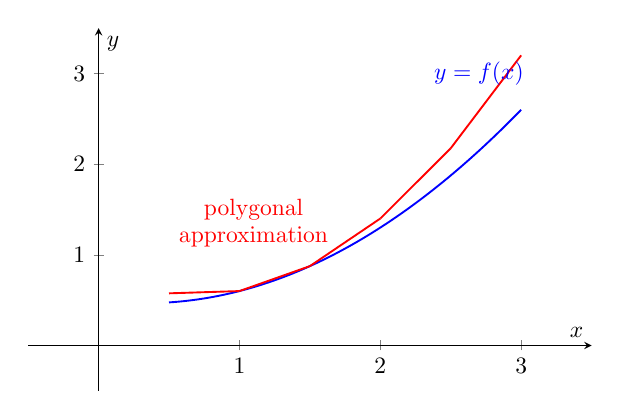
\begin{tikzpicture}[scale=0.85]
\begin{axis}[
axis lines=middle,
xlabel=$x$, ylabel=$y$,
xmin=-0.5, xmax=3.5,
ymin=-0.5, ymax=3.5,
xtick={1,2,3}, ytick={1,2,3},
width=10cm, height=7cm,
samples=100
]
\addplot[blue, thick, domain=0.5:3] {0.3*x^2 - 0.2*x + 0.5};
\draw[red, thick] (axis cs:0.5,0.575) -- (axis cs:1.0,0.6);
\draw[red, thick] (axis cs:1.0,0.6) -- (axis cs:1.5,0.875);
\draw[red, thick] (axis cs:1.5,0.875) -- (axis cs:2.0,1.4);
\draw[red, thick] (axis cs:2.0,1.4) -- (axis cs:2.5,2.175);
\draw[red, thick] (axis cs:2.5,2.175) -- (axis cs:3.0,3.2);
\node[blue] at (axis cs:2.7,3.0) {$y=f(x)$};
\node[red] at (axis cs:1.1,1.5) {polygonal};
\node[red] at (axis cs:1.1,1.2) {approximation};
\end{axis}
\end{tikzpicture}
\end{center}
\begin{example}
Find the length of the curve $y = x^{3/2}$ from $x = 0$ to $x = 4$.
$f'(x) = \frac{3}{2}\sqrt{x}$, so $[f'(x)]^2 = \frac{9}{4}x$. Thus,
\[
L = \int_0^4 \sqrt{1 + \frac{9}{4}x} \, dx.
\]
Let $u = 1 + \frac{9}{4}x$, $du = \frac{9}{4} dx$, so $dx = \frac{4}{9} du$. Limits: $x = 0 \to u = 1$, $x = 4 \to u = 10$.
\[
L = \frac{4}{9} \int_1^{10} \sqrt{u} \, du = \frac{4}{9} \cdot \frac{2}{3} [u^{3/2}]_1^{10} = \frac{8}{27} (10\sqrt{10} - 1) \approx 9.07.
\]
\end{example}
\begin{definition}[Arc Length for Parametric Curves]
If a curve is given parametrically by $x = f(t)$, $y = g(t)$ for $t \in [\alpha, \beta]$, where $f'$ and $g'$ are continuous, then the arc length is
\[
L = \int_{\alpha}^{\beta} \sqrt{[f'(t)]^2 + [g'(t)]^2} \, dt = \int_{\alpha}^{\beta} \sqrt{\left( \frac{dx}{dt} \right)^2 + \left( \frac{dy}{dt} \right)^2} \, dt.
\]
\end{definition}
\begin{example}
Find the length of the circle of radius $r$ parametrized by $x = r \cos t$, $y = r \sin t$ for $t \in [0, 2\pi]$.
$\frac{dx}{dt} = -r \sin t$, $\frac{dy}{dt} = r \cos t$. Thus,
\[
L = \int_0^{2\pi} \sqrt{r^2 \sin^2 t + r^2 \cos^2 t} \, dt = \int_0^{2\pi} r \, dt = 2\pi r.
\]
\end{example}
\begin{definition}[Arc Length of a Function of $y$]
If $x = g(y)$ with $g'$ continuous on $[c, d]$, then
\[
L = \int_c^d \sqrt{1 + [g'(y)]^2} \, dy.
\]
\end{definition}
\section{Areas of Surfaces of Revolution}
\begin{definition}[Surface Area about the $x$-Axis]
If $f$ is positive and has a continuous derivative on $[a, b]$, the area $S$ of the surface generated by revolving the curve $y = f(x)$ about the $x$-axis is
\[
S = \int_a^b 2\pi f(x) \sqrt{1 + [f'(x)]^2} \, dx.
\]
\end{definition}
\begin{proof}
Consider a small segment of arc length $\Delta s \approx \sqrt{1 + [f'(x)]^2} \Delta x$. When revolved about the $x$-axis, it generates a frustum of a cone with lateral area approximately $2\pi f(x) \Delta s$. Integrating gives the formula.
\end{proof}
\begin{center}
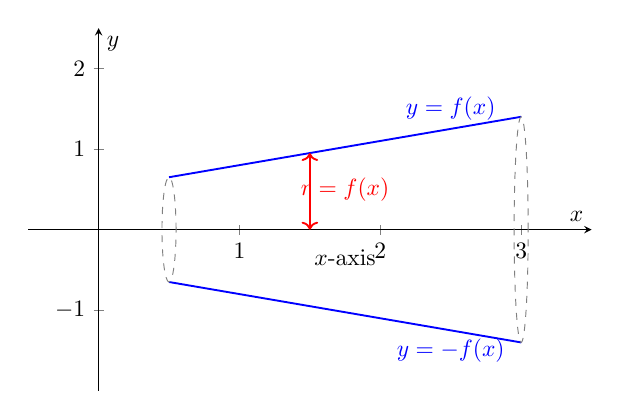
\begin{tikzpicture}[scale=0.85]
\begin{axis}[
axis lines=middle,
xlabel=$x$, ylabel=$y$,
xmin=-0.5, xmax=3.5,
ymin=-2.0, ymax=2.5,
xtick={1,2,3}, ytick={-1,1,2},
width=10cm, height=7cm,
samples=100
]
\addplot[blue, thick, domain=0.5:3] {0.3*x + 0.5};
\addplot[blue, thick, domain=0.5:3] {-0.3*x - 0.5};
\draw[dashed, gray] (axis cs:0.5,0) ellipse (0.05 and 0.65);
\draw[dashed, gray] (axis cs:3,0) ellipse (0.05 and 1.4);
\draw[<->, red, thick] (axis cs:1.5,0) -- (axis cs:1.5,0.95);
\node[red] at (axis cs:1.75,0.5) {$r=f(x)$};
\node[blue] at (axis cs:2.5,1.5) {$y=f(x)$};
\node[blue] at (axis cs:2.5,-1.5) {$y=-f(x)$};
\node at (axis cs:1.75,-0.35) {$x$-axis};
\end{axis}
\end{tikzpicture}
\end{center}
\begin{example}
Find the area of the surface generated by revolving $y = \sqrt{x}$ from $x = 1$ to $x = 4$ about the $x$-axis.
$f'(x) = \frac{1}{2\sqrt{x}}$, so $1 + [f'(x)]^2 = 1 + \frac{1}{4x} = \frac{4x + 1}{4x}$. Thus,
\[
S = \int_1^4 2\pi \sqrt{x} \cdot \sqrt{\frac{4x+1}{4x}} \, dx = \int_1^4 2\pi \sqrt{x} \cdot \frac{\sqrt{4x+1}}{2\sqrt{x}} \, dx = \pi \int_1^4 \sqrt{4x+1} \, dx.
\]
Let $u = 4x + 1$, $du = 4 \, dx$. Limits: $x = 1 \to u = 5$, $x = 4 \to u = 17$.
\[
S = \frac{\pi}{4} \int_5^{17} \sqrt{u} \, du = \frac{\pi}{4} \cdot \frac{2}{3} [u^{3/2}]_5^{17} = \frac{\pi}{6} (17\sqrt{17} - 5\sqrt{5}) \approx 30.85.
\]
\end{example}
\begin{definition}[Surface Area about the $y$-Axis]
If $g$ is positive and has a continuous derivative on $[c, d]$, the area $S$ of the surface generated by revolving the curve $x = g(y)$ about the $y$-axis is
\[
S = \int_c^d 2\pi g(y) \sqrt{1 + [g'(y)]^2} \, dy.
\]
\end{definition}
\begin{definition}[Surface Area for Parametric Curves]
If a curve is given parametrically by $x = f(t)$, $y = g(t)$ for $t \in [\alpha, \beta]$, with $g(t) \geq 0$ and $f'$, $g'$ continuous, the surface area generated by revolving about the $x$-axis is
\[
S = \int_{\alpha}^{\beta} 2\pi g(t) \sqrt{[f'(t)]^2 + [g'(t)]^2} \, dt.
\]
\end{definition}
\begin{example}
Find the surface area of a sphere of radius $r$.
The sphere is generated by revolving the semicircle $y = \sqrt{r^2 - x^2}$ for $x \in [-r, r]$ about the $x$-axis.
$f'(x) = \frac{-x}{\sqrt{r^2 - x^2}}$, so
\[
1 + [f'(x)]^2 = 1 + \frac{x^2}{r^2 - x^2} = \frac{r^2}{r^2 - x^2}.
\]
Thus,
\[
S = \int_{-r}^r 2\pi \sqrt{r^2 - x^2} \cdot \frac{r}{\sqrt{r^2 - x^2}} \, dx = 2\pi r \int_{-r}^r 1 \, dx = 2\pi r \cdot 2r = 4\pi r^2.
\]
\end{example}
\begin{definition}[General Surface Area Formula]
For a curve revolved about a horizontal line $y = c$,
\[
S = \int_a^b 2\pi |f(x) - c| \sqrt{1 + [f'(x)]^2} \, dx.
\]
For a curve revolved about a vertical line $x = c$,
\[
S = \int_c^d 2\pi |g(y) - c| \sqrt{1 + [g'(y)]^2} \, dy.
\]
\end{definition}
\begin{example}
Find the surface area generated by revolving $y = x^2$ on $[0, 1]$ about the $y$-axis.
Using the parametric form with $x = t$, $y = t^2$ for $t \in [0, 1]$. Then $\frac{dx}{dt} = 1$, $\frac{dy}{dt} = 2t$, and the distance from the $y$-axis is $x = t$. Thus,
\[
S = \int_0^1 2\pi t \sqrt{1 + 4t^2} \, dt.
\]
Let $u = 1 + 4t^2$, $du = 8t \, dt$, so $t \, dt = \frac{du}{8}$. Limits: $t = 0 \to u = 1$, $t = 1 \to u = 5$.
\[
S = 2\pi \cdot \frac{1}{8} \int_1^5 \sqrt{u} \, du = \frac{\pi}{4} \cdot \frac{2}{3} [u^{3/2}]_1^5 = \frac{\pi}{6} (5\sqrt{5} - 1) \approx 5.33.
\]
\end{example}
\begin{theorem}[Summary of Surface Area Formulas]
\begin{itemize}
\item About $x$-axis: $S = \displaystyle \int_a^b 2\pi y \sqrt{1 + \left( \frac{dy}{dx} \right)^2} \, dx$.
\item About $y$-axis: $S = \displaystyle \int_c^d 2\pi x \sqrt{1 + \left( \frac{dx}{dy} \right)^2} \, dy$.
\item Parametric about $x$-axis: $S = \displaystyle \int_{\alpha}^{\beta} 2\pi y(t) \sqrt{\left( \frac{dx}{dt} \right)^2 + \left( \frac{dy}{dt} \right)^2} \, dt$.
\item Parametric about $y$-axis: $S = \displaystyle \int_{\alpha}^{\beta} 2\pi x(t) \sqrt{\left( \frac{dx}{dt} \right)^2 + \left( \frac{dy}{dt} \right)^2} \, dt$.
\end{itemize}
\end{theorem}
\end{document}
